\documentclass[10pt,a4paper]{article}
\usepackage[utf8]{inputenc}
\usepackage{tikz}
\usepackage{pgfplots, pgfplotstable}
\usepackage{ae}
\usepackage[brazil]{babel}
\usepackage[vmargin=2cm,hmargin=2cm,columnsep=0.75cm]{geometry}
\usepackage{float,nonfloat}
\usepackage{graphicx,color}
\usepackage{subcaption}
\usepackage{amsmath}
\usepackage{verbatim}

\makeatletter
\let\@institution\empty
\def\institution#1{\def\@institution{#1}}
\renewcommand{\maketitle}{
    \begin{center}
        {\Large\bfseries\@title\par\medskip}
        {\large
            \begin{tabular}[t]{c}%
                \@author
        \end{tabular}\par\medskip}
        {\itshape\@institution\par}
        {\itshape\@date\par}
\end{center}}
\makeatother

\newcommand{\pixel}{\textit{pixel} }
\newcommand{\pixels}{\textit{pixels} }
\newcommand{\kernel}{\textit{kernel} }
\newcommand{\kernels}{\textit{kernels} }

\begin{document}
% ============================================================================

\title{MC920: Introdução ao Processamento de Imagem Digital\\Tarefa 12}
\author{
    \begin{minipage}{6cm}
        \centering
        Martin Ichilevici de Oliveira\\
        RA 118077
    \end{minipage}
    \and
    \begin{minipage}{6cm}
        \centering
        Rafael Almeida Erthal Hermano\\
        RA 121286
    \end{minipage}
}
\institution{Instituto de Computação, Universidade Estadual de Campinas}
\date{\today}

\maketitle

\section{Coerência direcional}
A coerência direcional mede o quão alinhadas estão as cristas de uma região da impressão digital. A coerência direcional pode ser definida como:

\begin{equation}
    coh = \frac{((G_{xx} - G_{yy})^2 + 4 * G_{xy}^2)^{\frac{1}{2}}}{G_{xx} - G_{yy}}
\end{equation}

\section{SVM}
Para classificar as regiões de tamanho $w$, foi utilizado o SVM(support vector machine) com o vetor de dados sendo a média, variância e coerência direcional da região. O SVM utilizada um kernel rbf e para treina-lo foram utilizadas 72 janelas de background e 98 janelas de foreground de tamanho $16$. Para validar o classificador foi utilizada a técnica de K-FOLD com 10 folds. A taxa de acerto esperada para o classificador com os dados de teste ficou em $0.90 \pm 0.004$

\section{Resultados}

\begin{figure}[!ht]
    \centering
    \begin{subfigure}[ht]{0.25\textwidth}
        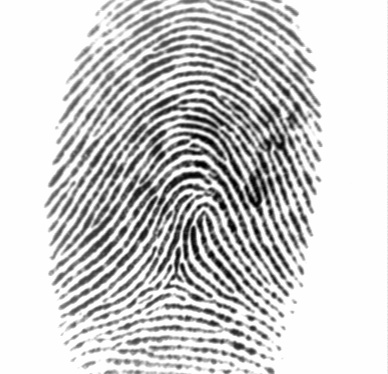
\includegraphics[width=\textwidth]{Fingerprints/1_1_rgnl.jpg}
        \caption{Imagem original}
    \end{subfigure}
    \qquad
    \begin{subfigure}[ht]{0.25\textwidth}
        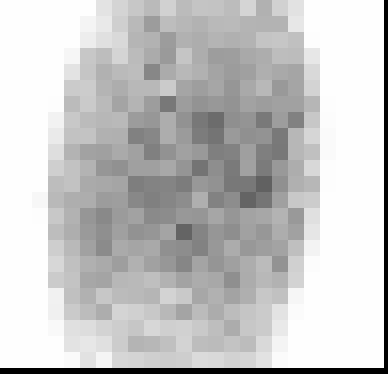
\includegraphics[width=\textwidth]{Fingerprints/1_1_mean.jpg}
        \caption{Média}
    \end{subfigure}
    \qquad
    \begin{subfigure}[ht]{0.25\textwidth}
        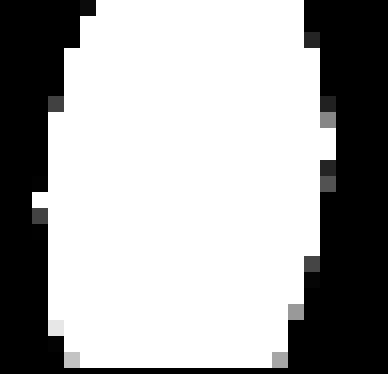
\includegraphics[width=\textwidth]{Fingerprints/1_1_vari.jpg}
        \caption{Varância}
    \end{subfigure}
    \qquad
    \begin{subfigure}[ht]{0.25\textwidth}
        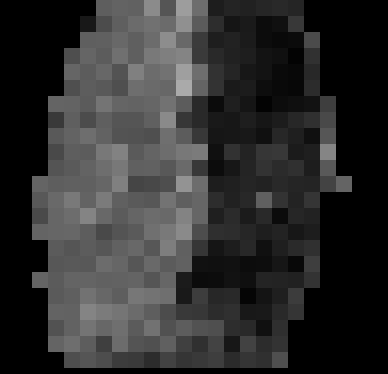
\includegraphics[width=\textwidth]{Fingerprints/1_1_cohe.jpg}
        \caption{Coerência direcional}
    \end{subfigure}
    \begin{subfigure}[ht]{0.25\textwidth}
        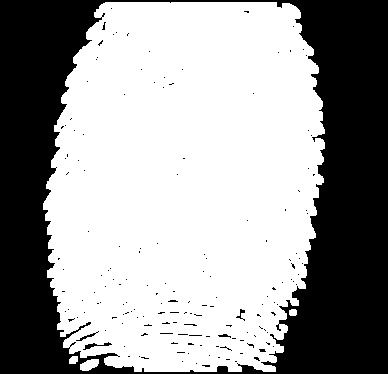
\includegraphics[width=\textwidth]{Fingerprints/1_1_filtered.jpg}
        \caption{FIltrada com SVM}
    \end{subfigure}
\end{figure}

\begin{thebibliography}{99}
    \bibitem{livro} GONZALEZ, Rafael C.; WOODS, Richard E.. \textbf{Digital Image Processing}. 3. ed. Upper Saddle River, NJ, EUA: Prentice-hall, 2006.
    \bibitem{artigo} BAZEN, Asker M.; GEREZ, Sabih H.. \textbf{Segmentation of fingerprint images}. ProRISC 2001 Workshop on Circuits, Systems and Signal Processing, 2011.
    
\end{thebibliography}
\end{document}
